\chapter{Introduction}
Where-are-my-parts (WAMP for short) is a simple intuitive game where the goal is to assemble broken robots in an efficient manner. The broken robot parts are scattered around the grid, where they can only move in 2D directions, till they hit an Obstacle, another part, or the border of the grid and die. Thenceforth, search algorithms were used to efficiently assemble the Robot with least possible cost. \\

WAMP has few limitations, for instance, the generated grid may not be solvable, due to the fact that robot parts must travel in a specific direction till it hits something, or die ( hits the grid wall). Furthermore, when two parts merge up, they occupy two grid blocks, thus bulk movements should be carefully managed. Finally, when a bulk of parts ( two or more merged robot parts) move together, the cost increases, which had to be handled in the heuristic part.\\

Java language was used in implementing the search problem. The project is divided into 9 main classes covering our approach implementation, the program is written for an external agent who controls the robot parts, the agent is aware of all parts' locations, obstacles and limitations, which is the main reason search algorithms are desirable for this kind of problems.\\

\textbf{Grid.java} : responsible for creating a random grid/problem, carry out cloning jobs and apply changes to the grid.

\textbf{SearchAlgorithm.java} : implements the general search algorithm discussed in the lecture.
\textbf{Heuristic.java }: calculates the heuristic value of a given node.

\textbf{Part.java} : ADT representing the robot part, including his location and neighbouring robot parts.

\textbf{SearchProblem.java} : an abstract class which represents the search problem discussed in the lecture.

\textbf{SearchTreeNode.java} : an abstract data type which represents the Search Tree node and structure discussed in the lecture. 

\textbf{Wamp.java} : extends Search algorithm class, it holds the algorithm implementation functions, the order of expansion queue and the main method.

\textbf{WampOperator.java} : represents the action/operator.

\textbf{WampSearchProblem.java} : extends SearchProblem, checks for goal test and calculates path cost.

\textbf{WampState.java} : represents a state in the state space.\\

The approach followed, the Abstract data types used and Heuristic implementation are discussed in more details next chapters.

\chapter{Implementation}


\section{ADT}
The \textit{SearchTreeNode} object can be represented as an ADT with six instance variables. The \textbf{state} this node corresponds to, the \textbf{parent node}, implemented by the same ADT, the \textbf{operator} applied to generate this node, the \textbf{depth} of the node in the tree, the \textbf{path cost} from the root and the \textbf{Heuristic} value of the node.\\

The \textit{SearchProblem} ADT is characterized by the following variables. The \textbf{State Space} containing all states reachable by any sequence of actions, the \textbf{initial state}, and list of \textbf{operators} available for the agent. Moreover, the goal test is computed by the function \textbf{boolean goalTest(State state)}, that takes a state as a parameter and checks if all parts are assembled or not. Also, it calculates the \textbf{pathcost(Objects... operators)} which takes a list of operators along with the initial state in the ADT, such that the path cost is returned for every state. Moreover, the class has \textit{transferFunction(State input, Operator operator)} that will generate the next possible state given any state and an operator.\\

Where-are-my-parts ADT is the main class, it extends search algorithm. It calls genGrid() to generate a grid with random width, height, number of robots and obstacles, the maximum size of the random grid is 8x8 for memory reasons, and minimum 3x3. After generating the grid, WAMP generate the list of operators and initialize the WAMP search problem. Moreover, Robot parts and obstacles count occupy 0\%-25\% of the area of the grid. After generating the grid, Wamp calls the search() method given the algorithm as an input to visualize a possible solution. Furthermore, the class holds all the algorithm implementation functions to be used whenever needed.

\section{Main Functions}
\subsubsection{GetBulkRec()}
GetBulkRec(Part p) is a function that returns all the Parts attached to the current part p and all the parts attached to them recursively . For simplicity, it gets all parts attached in a bulk if Part P is a subset of this bulk. 



\subsubsection{Transfer function()}
transferFunction(State input, Operator operator) generate the next possible state given any state and an operator. In other words, its the function responsible for moving the parts across the grid, checking the validity of the moves. 

\subsubsection{ApplyAndClone()}
ApplyAndClone(ArrayList<Part> AdjacentParts, WampOperator Operator,int partX, int partY) is used to apply changes to the current state after cloning it. It creates a new grid, clone the obstacles and robot parts, and apply changes on all AdjacentParts using the input Operator and the magnitude of the movement given(PartX,PartY). Furthermore, it gives the robot part some awareness of which part he merged with. Finally, it updates the grid by freeing the initial positions of the robot parts.

\subsubsection{GenGrid()}
GenGrid() generates a grid with random dimensions, robot parts' and obstacles locations.

\subsubsection{Search()}
Search(grid,strategy,visualise) manages the order of the expansion queue, checks the goal test, and call the various search algorithms implemented in WAMP.java. Finally, it prints and returns the solution and the steps to retrieve the final form, along with the path cost and number of expanded nodes. 


\chapter{Algorithms}
\section{Implementation}
\subsubsection{Breadth First Search}

A to-be-expanded queue is initialized at the beginning of the search approach, and the BFS function is called whenever this queue is nonempty. The function dequeues the first node from the beginning of the queue, expand it, and adds the expanded nodes to the end of the queue, till the goal test is satisfied or there is no solution (empty queue).

A simple adjustment to the algorithm has been implemented, as the repeated identical nodes are removed from the queue, due to the fact that the children would be identical as well because every part moves with his adjacent parts, and that will create redundant sub-problems when other parts try the same operator. 

\subsubsection{Depth First Search}

A to-be-expanded queue is initialized at the beginning of the search approach, and the DFS function is called whenever this queue is nonempty. The function dequeues the first node from the beginning of the queue, expand it, and adds the expanded nodes to the beginning of the queue, till the goal test is satisfied or there is no solution ( empty queue). 


\subsubsection{Iterative Deepening Search}

Iterative deepening simply sets a limit for the DFS function, thus, a limit is set at the beginning of the search, and the DFS function is called till the limit is reached, the goal test is satisfied or the queue get emptied.

\subsubsection{Greedy Search}
Greedy Search is set to expand the least heuristic valued node in the global queue of expanded nodes. Thus, the search dequeues the first value in the queue, expand it, and sort the children according to the heuristic value using insertion sort. It terminates if the goal test is achieved or the queue get emptied. However, due to the nature of the Where-are-my-parts problem, Robots can keep hitting an obstacle forever. This incompleteness gives the Greedy search an non-terminating manner in most cases.\footnote{Due to the nature of the problem, All search algorithms have non-terminating property, because when an object hits an obstacle using a specific operator, a new state is created with the same operator instead of ignoring it}

\subsubsection{A* Search}
The A* Search follows the same footsteps of the greedy. However, it takes to account the number of steps moved so far from the root node up to the current node as a part of the priority value in the queue. Thus, giving greedy search a completeness feature. i.e, a node with a robot hitting the wall will increase his priority queue value, putting it a step back for another node to try its luck.

\newpage
\section{Comparison}
\begin{figure}[H] 
   	\centering
	\includegraphics[scale=0.6]{images/Graph} 
    \caption{Implemented Algorithms vs Number of expanded nodes. (1000 represent infinity}
    \label{fig:graph} 
\end{figure}

\begin{figure}[H] 
   	\centering
	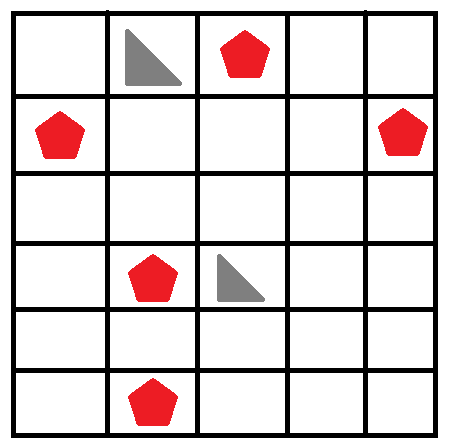
\includegraphics[scale=0.6]{images/grid} 
    \caption{Test case used.}
    \label{fig:grid} 
\end{figure}

As shown in graph \ref{fig:graph}, Breadth-First search and Iterative deepening share same Path cost. However, BF is more memory efficient as it expanded less number of nodes. The Greedy has the lowest number of expanded nodes due its features, with less path cost. However, Greedy algorithms are not complete in an unreliable way, such that, in most cases it tends not to terminate and find an answer. Finally, the A* search algorithm has the lowest optimum path cost from the initial state up to the goal state. However, the number of expanded nodes scales with the heuristic value and path cost, the lower the heuristic, the more nodes gets expanded.



\chapter{Heuristic}
\section{Centroid}

The Centroid approach was used and implemented as a heuristic function in the project. As in, The heuristic function returns the average distance between the robot parts in the grid and the centroid point between them. As illustrated in figure \ref{fig:centroid_model}, every robot parts' X and Y coordinates are modeled as a point in the grid. The points are used to create a virtual polygon by the aid of the geometry library "JTS". The Centroid is calculated using Polygon.getCentroid() function from JTS library. Finally, the average distance between all points and the centroid is returned as the heuristic value.

\begin{figure}[H] 
   	\centering
	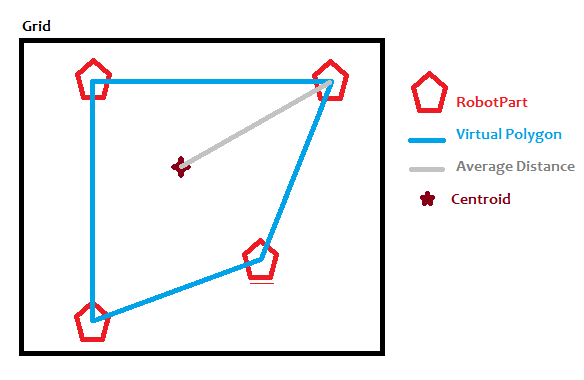
\includegraphics[scale=0.6]{images/Centroid} 
    \caption{Centroid concept illustration}
    \label{fig:centroid_model} 
\end{figure}

The heuristic approach proved to be a successful one, however it had a major drawback. If the Centroid can't be calculated because of the nature of the irregular shape e.g A twisted polygon as shown in figure \ref{fig:twistedcentroid}. The heuristic will return infinity. which wasn't acceptable. 

\begin{figure}[H] 
   	\centering
	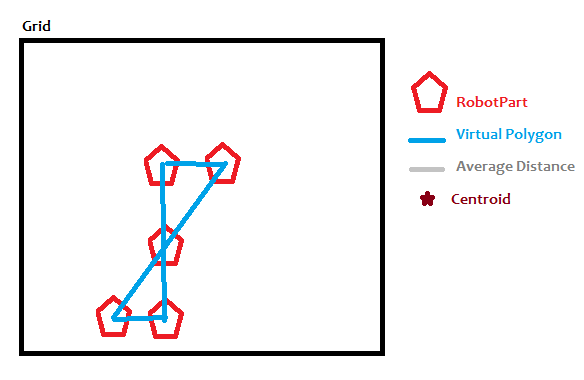
\includegraphics[scale=0.6]{images/twistedcentroid} 
    \caption{Centroid is incalculable incase of twisted polygons. }
    \label{fig:twistedcentroid} 
\end{figure}


\section{Average Distances}

Due to the Centroid unsuccessful attempt, the Average Distances approach was used. As in, it gets the summation of all the distances between all parts and each others as shown in figure \ref{fig:averagedistance}. The result is divided on the number of the parts Squared, to get an admissible Average Heuristic.

\begin{figure}[H] 
   	\centering
	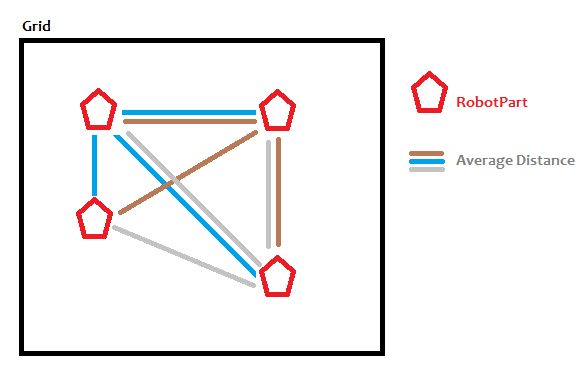
\includegraphics[scale=0.6]{images/averagedistance} 
    \caption{The distances between all parts and each other is used to evaluate the average distance. }
    \label{fig:averagedistance} 
\end{figure}

The heuristic approach is satisfying the \textbf{Centering} property. The heuristic function will check for merged up parts, returning a zero when all parts are conjoined, and returning the Average distance otherwise. \\

The approach followed is \textbf{consistent}. The heuristic value increases if one the parts stray away from the others, and decreases when it gains on other parts. The averaging is designed to get the Sum of distances and divide on the Number of parts squared. Thus, avoiding any chance for any overestimation of heuristic. Moreover, parts move in 2D grid, the average distance between 2 parts in a grid is the hypotenuse in most cases, which is always shorter than the catheti. In case of straight lines, the distance is the twice the same as the heuristic value (assuming distance is in unit steps), which proves \textbf{admissibility}.	


\section{Number of Bulks remaining}

The Number of Bulks remaining heuristic is a simple approach mainly used to assemble parts as fast as possible, The main concept is calculating the number of combined bulks of robot parts represented in the grid. Give more priority for small bulks to move, thus aiming to decrease the path cost by not moving the huge bulks. Also, it gives more priority for parts merging into other parts, rather than stopping at an obstacle.  \\

The heuristic function is calculated as follows, the size of the bulks in the grid is doubled and added. Thus, bigger bulks will have larger output. The output is inversed to satisfy the \textbf{Monotonic} property by giving the bigger bulks less heuristic values. The function returns the number of parts in the board divided by the inversed value to satisfy the \textbf{admissibility} property, as the heuristic will always be less than one ( the step cost). Finally, The \textbf{Centering} property is satisfied by a running check, returning a zero value if the number of bulks reaches one, i.e, there is only 1 merged robot.


\chapter{External Libraries}

The JTS Topology Suite is an opensource API of 2D spatial predicates and functions. JTS geometry library was used in the project to implement the Centroid and Average Distances Heuristics. \\

 Centroid was calculated as follows, every Robot Part's coordinates creates a new JTS \textbf{coordinates(double x,double y)}, which its used as a parameter for a \textbf{linearRing(Coordinates[] s)}, that creates the virtual \textbf{polygon(LinearRing r)}, the Centroid can be easily calculated using \textbf{Polygon.getCentroid()} which returns the centroid as a Point.\\
 
 Average Distances was calculated simply by using the following line, \textbf{DistanceOp. distance(Point x,Point y)}, where Point takes Coordinate as a parameter. Returns the average distance between two given points.
 \\
 
 
 